\documentclass{article}
\PassOptionsToPackage{numbers,compress}{natbib}
\usepackage[final]{neurips}
\usepackage[utf8]{inputenc}
\usepackage[T1]{fontenc}
\usepackage{booktabs}
\usepackage{amsmath,amsfonts,amssymb}
\usepackage{graphicx}
\usepackage{microtype}
\usepackage{xcolor}
\usepackage{array}
\usepackage{float}
\usepackage{enumitem}
\usepackage{tikz}
\usetikzlibrary{arrows.meta,positioning}
\usepackage[hidelinks]{hyperref}
\setlist{nosep,leftmargin=*}
\setlength{\textfloatsep}{5pt plus 1pt minus 1pt}
\setlength{\floatsep}{4pt plus 1pt minus 1pt}
\setlength{\intextsep}{4pt plus 1pt minus 1pt}
\newcommand{\R}{\mathbb{R}}

\title{SRUL: Spatial Spherical Latents with Riemannian Flow Matching}
\author{Mohammadreza Tavasoli Naeini \\
Department of Electrical and Computer Engineering, University of Toronto \\
\texttt{mohammadreza.tavasolinaeini@mail.utoronto.ca}}

\begin{document}
\maketitle

\begin{abstract}
Autoencoder latents are often modeled with Gaussian priors, although their learned geometry depends on the architecture and regularization. Normalized encoders can produce nearly fixed-radius representations, with Transformer encoders using LayerNorm as one important example. For these latents, a Gaussian source introduces radial variation that the encoder does not use; even after normalizing the endpoints, straight Euclidean interpolation forms a chord through the sphere's interior. We propose \emph{Spherical Riemannian Unified Latents} (SRUL), which learns a spatial grid of spherical tokens and models their distribution with Riemannian Flow Matching (RFM). A spherical source, geodesic paths, and tangent-projected velocities keep generation on the same manifold, while tangent noise controls angular perturbation. On CIFAR-10, replacing the chord by RFM improves FID from $67.44$ to $63.84$ with the same spherical encoder and decoder. A noise sweep selects $\sigma_{\mathrm{enc}}=0.05$, and conditional sampling reaches FID $48.71$. The same pipeline is also evaluated on PathMNIST and CelebA-64.
\end{abstract}

\section*{Attestation of Teamwork}
Mohammadreza Tavasoli Naeini conducted the background study, designed and implemented the models, ran and analyzed the experiments, and prepared the report, presentation, and code.

\section{Introduction}
Latent generative models first map images to a compact code and then learn a prior over that code. Gaussian geometry is common, but an autoencoder does not guarantee it. Normalized encoders can instead produce nearly fixed-radius features, with Transformer encoders using LayerNorm as one example. Ignoring the learned affine parameters, a $C$-dimensional LayerNorm token satisfies $\|\operatorname{LN}(h)\|_2^2\approx C$, so radial variation is small and much of the information can be carried by direction \cite{rjf}. Explicit feature normalization can create the same structure in other encoders. SRUL makes it exact by normalizing every spatial latent token to unit norm.

Because every SRUL token has fixed radius, a Gaussian source introduces a radial degree of freedom that the representation does not use. Normalizing only the source and target endpoints is still insufficient: linear Euclidean interpolation between them follows a chord and creates intermediate states inside the sphere. The decomposition
\begin{equation}
\mathbb E_x\!\left[\mathrm{KL}\big(q_\phi(z\mid x)\|p(z)\big)\right]
= I_q(X;Z)+\mathrm{KL}\big(q_\phi(z)\|p(z)\big)
\label{eq:kl}
\end{equation}
separates the information stored in the latent from the mismatch between the aggregate encoder distribution and the prior. After the information level is fixed, matching the prior support and the transport path to the product-of-spheres geometry avoids modeling unused radial variation and off-manifold states. This motivates a spherical source together with geodesic transport.

The project asks a focused question: \emph{when the encoder produces spherical latent tokens, should the prior move through the sphere or along its surface?} We make three contributions. First, we learn a spatial product-of-spheres representation that preserves local image structure. Second, we use RFM so that the probability path, velocity field, and numerical integration remain on the same manifold. Third, we study tangent-noise scale and classifier-free guidance as separate controls, and evaluate the same pipeline on CIFAR-10, PathMNIST, and CelebA-64.

\section{Related Work and Positioning}
Latent Diffusion Models (LDMs) move generation from pixels to a learned Euclidean latent grid, which reduces computation while preserving perceptually important information \cite{ldm}. Unified Latents studies how encoder noise controls the amount of information passed through the latent representation, but its generative process remains Euclidean \cite{ul}. Sphere Encoder explicitly maps images to a sphere and trains the decoder to remain stable around encoded points, with the goal of direct sampling from an approximately uniform spherical distribution \cite{sphere}.

Flow Matching learns a time-dependent velocity field along a chosen probability path \cite{fm}. RJF observes that normalized representation encoders often produce nearly fixed-radius features and replaces Euclidean interpolation with Riemannian Flow Matching on the sphere; it also studies an additional Jacobi weighting \cite{rjf}. SRUL builds on these directions but learns the representation and prior together as one pipeline. It uses a spatial spherical autoencoder, applies controlled tangent perturbations, and learns the nonuniform distribution of encoded tokens with an RFM prior. Unlike direct spherical sampling, the model does not assume that all points on the product of spheres are equally probable.

\section{Method}
\subsection{Pipeline overview}
Figure~\ref{fig:pipeline} shows the complete SRUL pipeline. Representation learning produces a grid of unit-norm tokens and trains the decoder to remain stable under tangent perturbations. RFM then learns the distribution of these encoded tokens using geodesic paths and tangent velocities. During sampling, spherical noise is transported with exponential-map steps and decoded into a new image.

\begin{figure}[H]
\centering
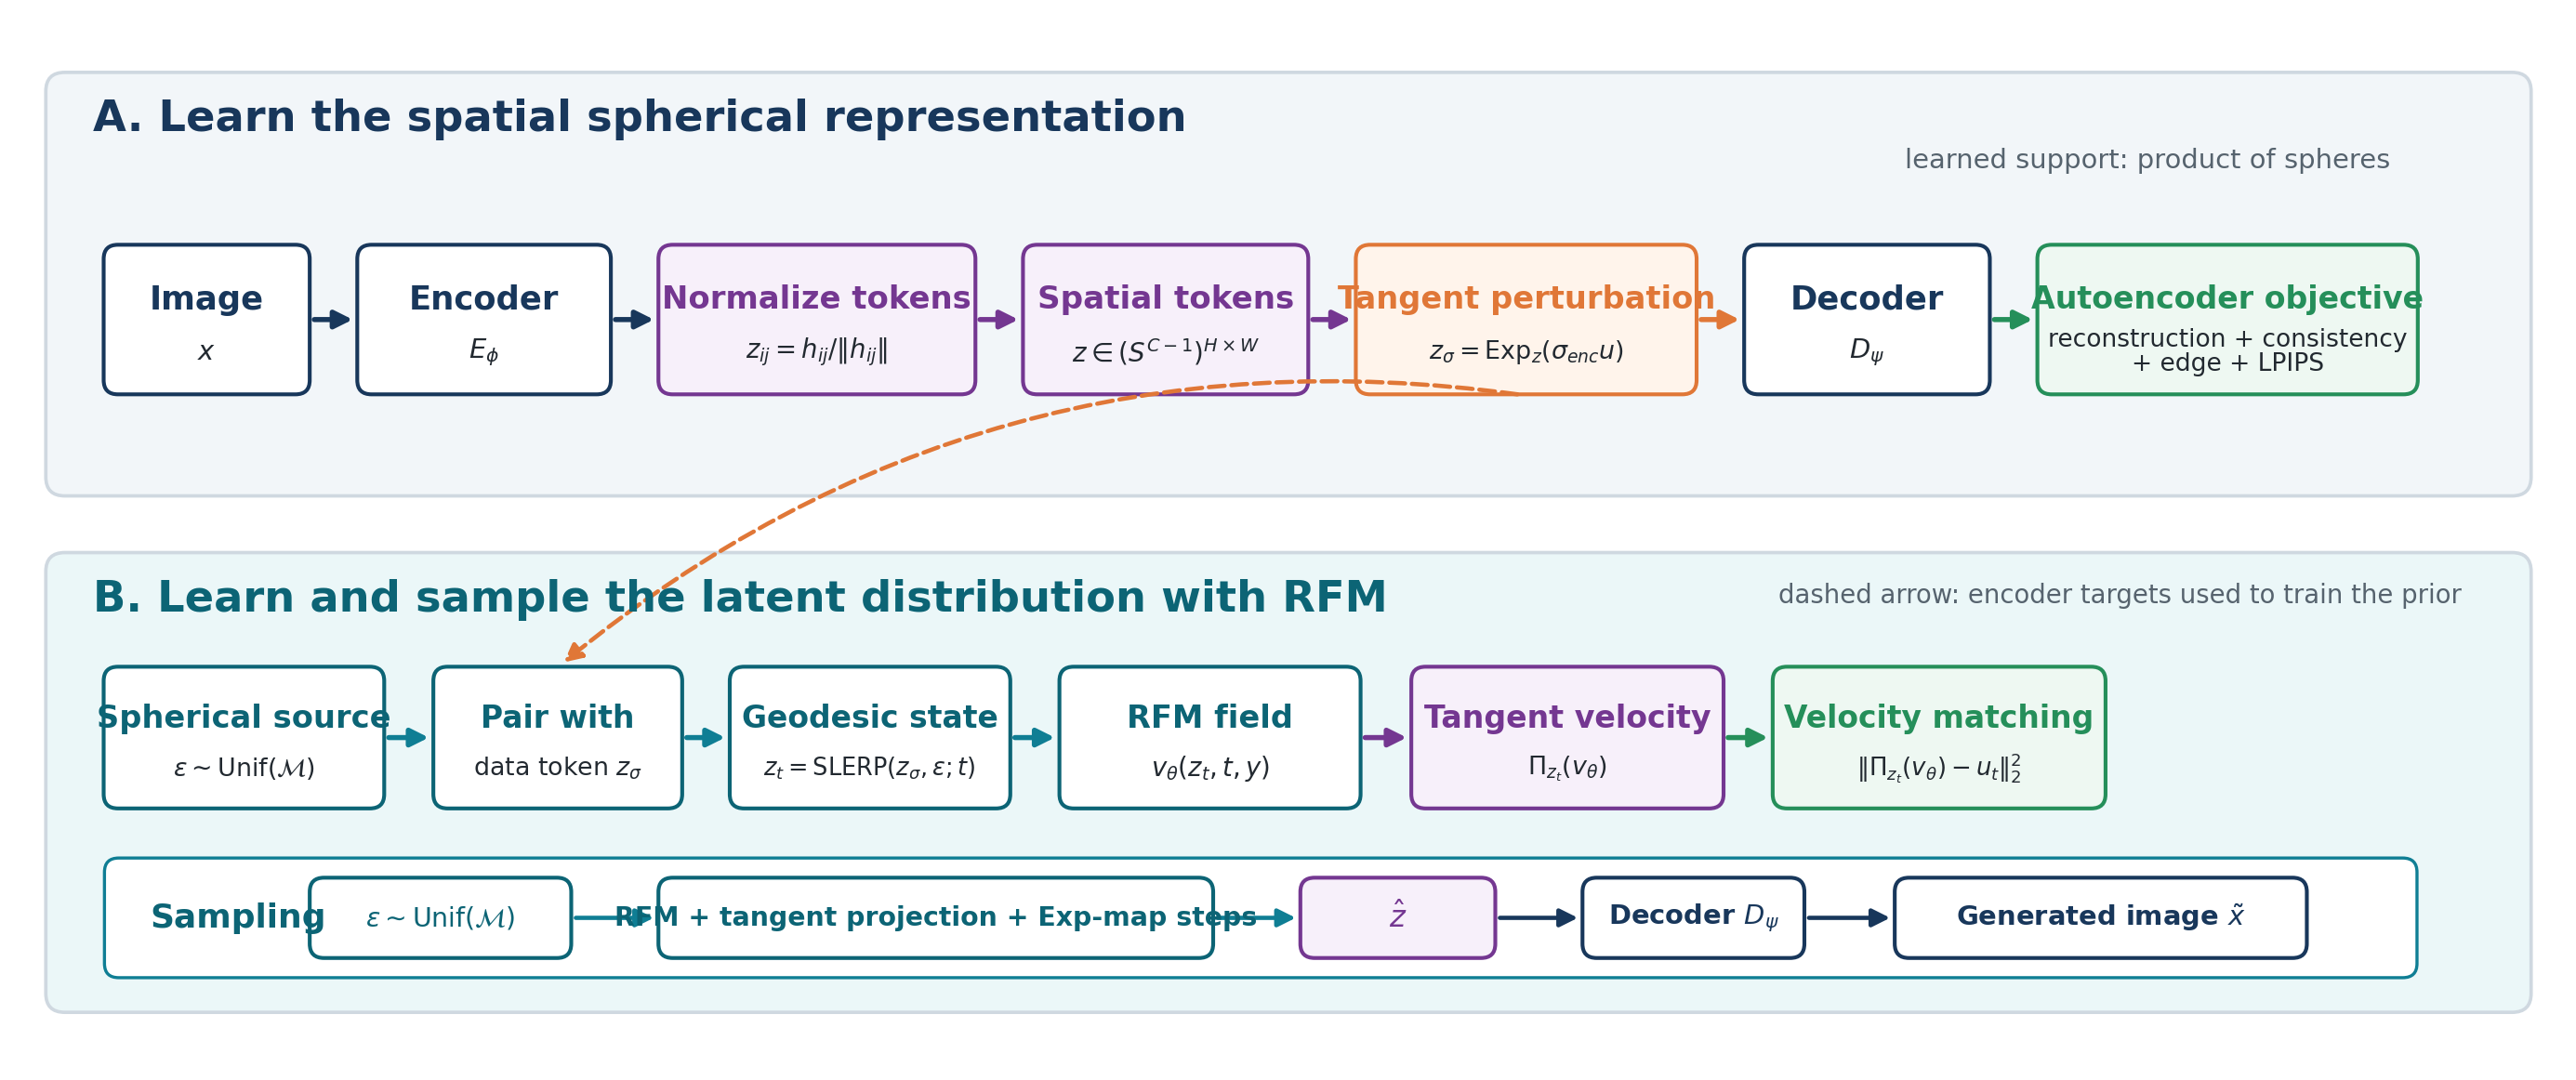
\includegraphics[width=0.99\linewidth]{assets/srul_pipeline_v10.png}
\caption{SRUL pipeline. The top stage learns spatial spherical tokens and a decoder robust to tangent perturbations. The lower stage trains and samples an RFM prior on the same product-of-spheres manifold. Class labels and classifier-free guidance are optional conditional inputs.}
\label{fig:pipeline}
\end{figure}

\subsection{Spatial spherical autoencoder}
For an image $x$, the encoder produces a spatial tensor
\begin{equation}
 h=E_\phi(x)\in\R^{C\times H\times W},\qquad
 z_{:,i,j}=\frac{h_{:,i,j}}{\|h_{:,i,j}\|_2}\in S^{C-1}.
\label{eq:encoder}
\end{equation}
The full latent space is the product manifold $\mathcal M=(S^{C-1})^{HW}$. We use $C=32$, a $4\times4$ token grid for $32\times32$ images, and an $8\times8$ grid for CelebA-64. The spatial layout allows different tokens to retain local image information, while normalization removes the radial degree of freedom.

The autoencoder is trained from clean and perturbed latents:
\begin{align}
\mathcal L_{\mathrm{AE}}={}&
\lambda_c\|D_\psi(z)-x\|_1
+\lambda_n\|D_\psi(z_\sigma)-x\|_1
+\lambda_e\mathcal L_{\mathrm{edge}} \nonumber\\
&+\lambda_{\mathrm{lat}}\big[1-\cos\big(z,E_\phi(D_\psi(z_\sigma))\big)\big]
+\lambda_p\mathcal L_{\mathrm{LPIPS}}.
\label{eq:ae}
\end{align}
The clean and noisy reconstruction terms preserve image content, while latent consistency, edge loss, and LPIPS improve local stability and perceptual detail.

\subsection{Tangent-noise control}
For each token, Gaussian noise is projected onto the tangent space,
\begin{equation}
 \xi\sim\mathcal N(0,I),\qquad
 u=\Pi_z(\xi)=\xi-\langle\xi,z\rangle z,
\end{equation}
and the perturbed token is
\begin{equation}
 z_\sigma=\operatorname{Exp}_z(\sigma_{\mathrm{enc}}u).
\label{eq:noise}
\end{equation}
Because $u\perp z$, the operation changes direction without changing radius. The scalar $\sigma_{\mathrm{enc}}$ therefore gives direct control over angular perturbation and retained image information.

\subsection{Riemannian Flow Matching prior}
The source is uniform on the same manifold, $\epsilon\sim\operatorname{Unif}(\mathcal M)$. For a data latent $z_\sigma$ and source sample $\epsilon$, the tokenwise geodesic is
\begin{equation}
 z_t=\operatorname{SLERP}(z_\sigma,\epsilon;t)
 =\frac{\sin((1-t)\Omega)}{\sin\Omega}z_\sigma
 +\frac{\sin(t\Omega)}{\sin\Omega}\epsilon,
\quad \Omega=\arccos(z_\sigma^\top\epsilon).
\label{eq:slerp}
\end{equation}
Let $u_t=\partial z_t/\partial t$ be the target tangent velocity. We train
\begin{equation}
 \mathcal L_{\mathrm{RFM}}
 =\mathbb E\!\left[\left\|\Pi_{z_t}\big(v_\theta(z_t,t)\big)-u_t\right\|_2^2\right].
\label{eq:rfm}
\end{equation}
During sampling, each predicted velocity is projected and integrated with the exponential map,
\begin{equation}
 z_{t-\Delta t}=\operatorname{Exp}_{z_t}\!\left(-\Delta t\,\Pi_{z_t}(v_\theta)\right),
\label{eq:sample}
\end{equation}
so every intermediate token remains on its sphere.

\subsection{Conditional generation and classifier-free guidance}
Conditioning is added without changing the spherical geometry. The field receives a label $y$, giving $v_\theta(z_t,t,y)$. During training, the label is replaced by a null label with probability $0.1$. During sampling,
\begin{equation}
 v_{\mathrm{CFG}}=v_\theta(z_t,t,\varnothing)
+s\big[v_\theta(z_t,t,y)-v_\theta(z_t,t,\varnothing)\big].
\label{eq:cfg}
\end{equation}
The guided field is projected onto the tangent space before every exponential-map update. CFG therefore changes conditional sampling strength but not the manifold or probability path.

\section{Experiments}
\subsection*{Setup}
CIFAR-10 is used for controlled comparisons \cite{cifar}. PathMNIST tests transfer to texture-dominated histopathology \cite{medmnist}, and CelebA-64 tests higher-resolution facial structure \cite{celeba}. AdamW is used in both training stages, and final samples use 100 integration steps. We report FID and KID for distribution quality, feature precision and recall for fidelity and coverage, and token norm for geometry.

\begin{table}[H]
\centering
\small
\caption{Datasets and model configurations.}
\label{tab:setup}
\setlength{\tabcolsep}{5.5pt}
\begin{tabular}{lrrrrl}
\toprule
Dataset & Train & Resolution & Token grid & AE/prior epochs & Conditioning \\
\midrule
CIFAR-10 & 50,000 & $32^2$ & $4\times4$ & 60/120 & class label \\
PathMNIST & 89,996 & $32^2$ & $4\times4$ & 50/80 & tissue class \\
CelebA-64 & 30,000 & $64^2$ & $8\times8$ & 40/60 & smiling attribute \\
\bottomrule
\end{tabular}
\end{table}

\subsection*{Does the transport path match the encoder geometry?}
The main comparison keeps the spherical encoder, decoder, source distribution, latent size, prior capacity, and training budget fixed. Only the path changes. The baseline uses
\begin{equation}
 z_t^{\mathrm{chord}}=(1-t)z_\sigma+t\epsilon.
\end{equation}
Although both endpoints have unit norm, the chord enters the sphere. For nearly orthogonal endpoints, its midpoint has norm $\|(z_\sigma+\epsilon)/2\|_2\approx1/\sqrt2=0.707$. The measured minimum mean norm is $0.705$. SRUL instead follows SLERP and remains at norm $1$.

\begin{figure}[H]
\centering
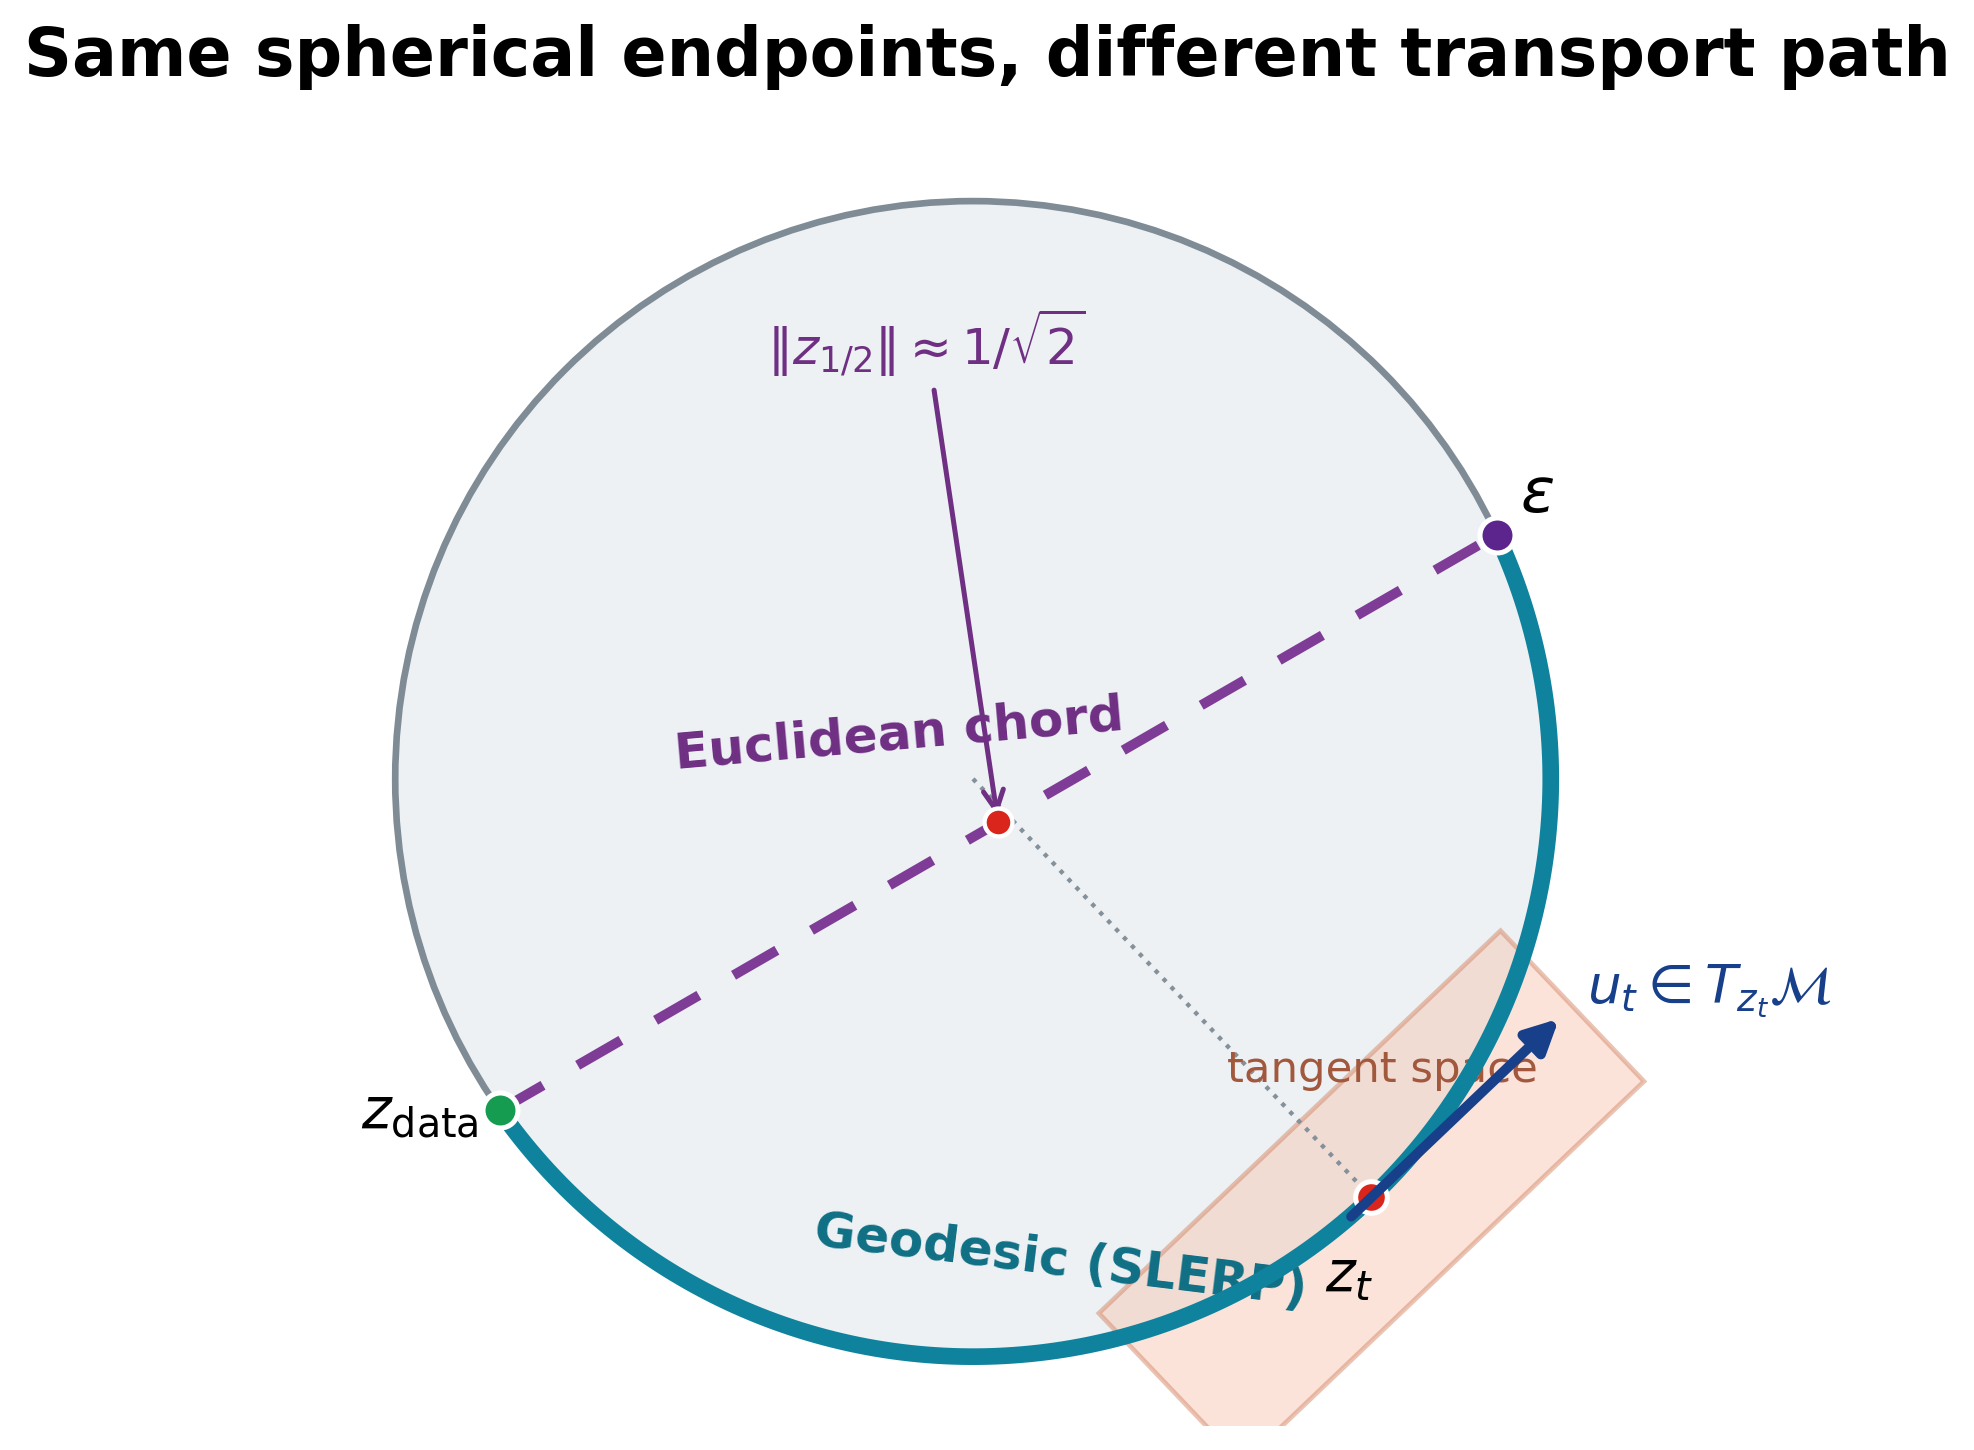
\includegraphics[width=0.64\linewidth]{assets/geometry_schematic_v9_clean.png}
\caption{The chord visits interior states that the spherical encoder does not produce. SRUL follows the geodesic, and its velocity lies in the tangent space.}
\label{fig:geometry}
\end{figure}

\begin{table}[H]
\centering
\small
\caption{CIFAR-10 controlled comparison with the same spherical encoder and decoder.}
\label{tab:geometry}
\setlength{\tabcolsep}{8.0pt}
\begin{tabular}{lrrrrr}
\toprule
Method & FID$\downarrow$ & KID$\downarrow$ & Precision$\uparrow$ & Recall$\uparrow$ & Min. norm$\uparrow$ \\
\midrule
Chord baseline & 67.44 & 0.0740 & 0.840 & 0.085 & 0.705 \\
\textbf{SRUL} & \textbf{63.84} & \textbf{0.0667} & \textbf{0.857} & \textbf{0.091} & \textbf{1.000} \\
\bottomrule
\end{tabular}
\end{table}

The geodesic path improves all four image metrics and removes the radial excursion. This supports the central hypothesis: once the representation is spherical, its generative transport should remain on the manifold.

\subsection*{Control ablations}
We train a separate conditional SRUL prior for each tangent-noise value. Increasing $\sigma_{\mathrm{enc}}$ removes more image information and worsens both reconstruction and generation; $0.05$ is the best tested value. We then vary CFG while keeping the representation and RFM objective fixed. Stronger guidance improves FID and precision, but reduces recall.

\begin{table}[H]
\centering
\small
\caption{CIFAR-10 tangent-noise and classifier-free-guidance ablations.}
\label{tab:controls}
\setlength{\tabcolsep}{5.5pt}
\begin{tabular}{crrr|crrr}
\toprule
$\sigma_{\mathrm{enc}}$ & Recon. FID$\downarrow$ & Gen. FID$\downarrow$ & Recall$\uparrow$ & CFG $s$ & FID$\downarrow$ & Precision$\uparrow$ & Recall$\uparrow$ \\
\midrule
0.05 & \textbf{17.53} & \textbf{48.71} & 0.090 & 1.0 & 62.44 & 0.854 & \textbf{0.083} \\
0.15 & 19.56 & 51.61 & \textbf{0.090} & 1.5 & 54.83 & 0.865 & 0.071 \\
0.30 & 27.85 & 58.16 & 0.073 & 2.0 & \textbf{49.39} & \textbf{0.884} & 0.059 \\
\bottomrule
\end{tabular}
\end{table}

\subsection*{Evaluation across image domains}
We applied the same spatial spherical representation and RFM prior in three settings. CIFAR-10 provides the controlled geometry and sampling ablations, PathMNIST evaluates local histopathology texture, and CelebA-64 tests a larger token grid on structured facial images. Table~\ref{tab:domains} summarizes the selected configuration and its quantitative results in each setting.

\begin{table}[H]
\centering
\small
\caption{Selected SRUL results in three evaluation settings. Reconstruction and generation metrics are computed against the real split of the corresponding dataset.}
\label{tab:domains}
\setlength{\tabcolsep}{3.2pt}
\renewcommand{\arraystretch}{1.12}
\begin{tabular}{p{1.35cm}p{3.15cm}p{2.35cm}rrrr}
\toprule
Dataset & Evaluation setting & Grid / selected controls & Recon. FID & Gen. FID & Precision & Recall \\
\midrule
CIFAR-10 & Natural-object geometry and sampling study & $4\times4$; $\sigma_{\mathrm{enc}}=0.05$, $s=2$ & 17.53 & 48.71 & 0.861 & 0.090 \\
PathMNIST & Texture-dominated histopathology transfer & $4\times4$; $\sigma_{\mathrm{enc}}=0.15$, $s=2$ & 7.13 & 29.36 & 0.829 & 0.309 \\
CelebA-64 & $64\times64$ facial-image scale-up & $8\times8$; $\sigma_{\mathrm{enc}}=0.15$, $s=2$ & 9.08 & 41.22 & 0.657 & 0.198 \\
\bottomrule
\end{tabular}
\end{table}

On CIFAR-10, the selected result follows the controlled chord-versus-geodesic comparison and the noise and guidance ablations. PathMNIST shows that the same $4\times4$ token design can model fine tissue texture. CelebA-64 increases the latent grid to $8\times8$ and preserves coherent facial structure at twice the image resolution.


\section{Conclusion}
SRUL learns spatial spherical tokens and models them with an RFM prior. With the encoder and decoder fixed, replacing the Euclidean chord by a geodesic improves CIFAR-10 FID from $67.44$ to $63.84$ and keeps every token on the manifold. The best tested noise scale is $\sigma_{\mathrm{enc}}=0.05$, and classifier-free guidance provides a separate fidelity--diversity control. PathMNIST and CelebA-64 show that the same design transfers to tissue texture and higher-resolution faces.

\clearpage
{\small
\begin{thebibliography}{9}
\bibitem{ldm} R. Rombach, A. Blattmann, D. Lorenz, P. Esser, and B. Ommer. High-resolution image synthesis with latent diffusion models. CVPR, 2022.
\bibitem{fm} Y. Lipman, R. T. Q. Chen, H. Ben-Hamu, M. Nickel, and M. Le. Flow matching for generative modeling. ICLR, 2023.
\bibitem{rjf} A. Kumar and V. M. Patel. Learning on the Manifold: Unlocking Standard Diffusion Transformers with Representation Encoders. arXiv, 2026.
\bibitem{sphere} Z. Yue et al. Image Generation with a Sphere Encoder. arXiv, 2026.
\bibitem{ul} J. Heek et al. Unified Latents: Controlling Information Flow in Latent Generative Models. arXiv, 2026.
\bibitem{cifar} A. Krizhevsky. Learning Multiple Layers of Features from Tiny Images. Technical report, 2009.
\bibitem{medmnist} J. Yang, R. Shi, D. Wei, et al. MedMNIST v2: A Large-Scale Lightweight Benchmark for 2D and 3D Biomedical Image Classification. Scientific Data, 2023.
\bibitem{celeba} Z. Liu, P. Luo, X. Wang, and X. Tang. Deep Learning Face Attributes in the Wild. ICCV, 2015.
\end{thebibliography}}
\end{document}
